\documentclass[aspectratio=169,11pt]{beamer}
% ==================================================================
% LogicWard — Pitch Deck  (Beamer -> PDF)
% Compile:  pdflatex LogicWard_Pitch_Deck.tex   (run twice)
% ==================================================================
\usepackage[T1]{fontenc}
\usepackage{lmodern}
\usepackage{tikz}
\usetikzlibrary{arrows.meta,positioning,fit,backgrounds,calc}
\usepackage{booktabs}
\usepackage{tabularx}

\usetheme{default}
\usefonttheme{professionalfonts}
\setbeamertemplate{navigation symbols}{}
\setbeamertemplate{itemize items}[circle]

% ---------------- palette ----------------
\definecolor{navy}{HTML}{14304F}
\definecolor{navy2}{HTML}{1D4370}
\definecolor{accent}{HTML}{3987E5}
\definecolor{ink}{HTML}{1F2937}
\definecolor{muted}{HTML}{5B6B80}
\definecolor{good}{HTML}{0E7A0E}
\definecolor{serious}{HTML}{C05621}
\definecolor{critical}{HTML}{C02626}
\definecolor{chem}{HTML}{A16207}
\definecolor{page}{HTML}{EEF0F4}
\definecolor{hair}{HTML}{DBE0E8}

\setbeamercolor{normal text}{fg=ink}
\setbeamercolor{frametitle}{fg=navy}
\setbeamercolor{title}{fg=white}
\setbeamercolor{structure}{fg=accent}
\setbeamercolor{itemize item}{fg=accent}
\setbeamercolor{itemize subitem}{fg=muted}
\setbeamercolor{block title}{fg=white,bg=navy}
\setbeamercolor{block body}{fg=ink,bg=page}
\setbeamerfont{frametitle}{series=\bfseries,size=\Large}
\setbeamerfont{title}{series=\bfseries}

% accent rule under each frame title
\setbeamertemplate{frametitle}{%
  \vspace{4pt}\hspace{2pt}\insertframetitle\\[-2pt]
  {\color{accent}\rule{0.14\paperwidth}{2.2pt}}\vspace{-2pt}}

\newcommand{\hl}[1]{{\color{accent}\textbf{#1}}}
\newcommand{\code}[1]{{\ttfamily\small #1}}
\tikzset{
  box/.style={rectangle,rounded corners=2pt,draw=navy!70,fill=navy!5,line width=0.6pt,
              text=ink,align=center,font=\scriptsize\sffamily,inner sep=4pt,minimum height=8mm},
  acc/.style={box,draw=accent,fill=accent!8},
  red/.style={box,draw=critical,fill=critical!8},
  chemb/.style={box,draw=chem,fill=chem!10},
  goodb/.style={box,draw=good,fill=good!10},
  fl/.style={-{Latex[length=2mm]},line width=0.7pt,draw=navy2},
  flr/.style={-{Latex[length=2mm]},line width=0.7pt,draw=critical},
  lbl/.style={font=\tiny\sffamily,text=muted,fill=white,inner sep=1pt},
}

% ==================================================================
\begin{document}

% ---------------- TITLE ----------------
{
\setbeamertemplate{background}{\color{navy}\rule{\paperwidth}{\paperheight}}
\setbeamercolor{normal text}{fg=white}
\begin{frame}[plain]
\vspace{0.8cm}
{\color{accent}\rule{0.5\textwidth}{2.5pt}}\\[10pt]
{\Huge\bfseries\color{white} LogicWard}\\[6pt]
{\large\color{page} Live OT Drift-Detection \& Incident-Response Platform}\\[16pt]
{\color{page}\small One detection fabric. Two live plants. Twelve real attacks.}\\[4pt]
{\color{page}\small A thermal power plant on a Raspberry Pi \textbf{+} a chemical reactor as a live 3D twin ---}\\
{\color{page}\small monitored, attacked, detected and rolled back under one SOC console.}\\[22pt]
{\color{muted}\footnotesize Adani OT Cybersecurity Demonstration}
\end{frame}
}

% ---------------- PROBLEM ----------------
\begin{frame}{The problem: OT attacks are invisible until they hurt}
\begin{columns}[T]
\begin{column}{0.56\textwidth}
\begin{itemize}
  \item IT security assumes patchable, restartable, observable assets. \hl{OT inverts every assumption.}
  \item Modbus has \hl{no authentication}. A PLC cannot be patched mid-process; a ``reboot'' can trip the plant.
  \item The adversary's goal is not data --- it is \hl{physical consequence}: defeat a safety interlock, then let physics do the damage.
  \item A lowered trip setpoint or an inverted safety comparator can sit \hl{invisibly} in a running plant for weeks.
\end{itemize}
\end{column}
\begin{column}{0.42\textwidth}
\begin{block}{The gap}
\small You cannot defend what you cannot \emph{see}. Operators watch process values --- not whether the \emph{control logic itself} still matches what was approved.
\end{block}
\vspace{4pt}
{\color{muted}\footnotesize Ukraine 2015/16, TRITON/TRISIS, and Oldsmar all began as unauthorized changes to trusted OT devices.}
\end{column}
\end{columns}
\end{frame}

% ---------------- SOLUTION ----------------
\begin{frame}{LogicWard: detect drift before it becomes risk}
\begin{block}{One sentence}
\small LogicWard watches the \hl{running control logic} and the \hl{live process state}, and raises \hl{severity-ranked, MITRE-mapped, evidence-backed} alerts the instant either drifts from a cryptographically signed, approved baseline.
\end{block}
\vspace{6pt}
\begin{columns}[T]
\begin{column}{0.5\textwidth}
\textbf{\color{navy}What makes it credible}
\begin{itemize}\small
  \item Detection is a structural \hl{diff}, not anomaly-guessing --- \hl{zero false positives}.
  \item The PLC program is \hl{data to diff, never executed}.
  \item HMAC-signed baseline: tamper breaks the signature.
\end{itemize}
\end{column}
\begin{column}{0.5\textwidth}
\textbf{\color{navy}What makes it win}
\begin{itemize}\small
  \item \hl{Multi-site, multi-vendor} --- one fabric, two very different plants.
  \item A live \hl{3D digital twin} of the chemical reactor.
  \item Production-grade SOC: risk, timeline, health, rollback.
\end{itemize}
\end{column}
\end{columns}
\end{frame}

% ---------------- TWO PLANTS ----------------
\begin{frame}{Two plants, one detection fabric}
\begin{columns}[T]
\begin{column}{0.5\textwidth}
\begin{block}{Site A --- Thermal Power Plant}
\small
\textbf{Raspberry Pi} (real hardware)\\
Rockwell \textbf{L5X} ladder logic\\
Structural \emph{+} register detection\\
Animated SVG SCADA mimic\\
\code{thermal-pi} \textbullet\ Modbus :5020
\end{block}
\end{column}
\begin{column}{0.5\textwidth}
\begin{block}{Site B --- GRFICS Chemical Reactor}
\small
\textbf{Live Unity 3D} digital twin\\
OpenPLC \textbf{Structured Text}\\
Register-plane detection\\
Reactor + gauges + explosion\\
\code{grfics-chem} \textbullet\ Modbus :5021
\end{block}
\end{column}
\end{columns}
\vspace{8pt}
\begin{center}\small
\hl{The claim:} not ``I detect drift on my simulator'' --- but ``I detect drift across \emph{vendors,
languages and processes} on one fabric.'' A new plant is a \emph{site profile}, not a rewrite.
\end{center}
\end{frame}

% ---------------- ARCHITECTURE ----------------
\begin{frame}{Architecture: one enriched event bus is the spine}
\begin{center}
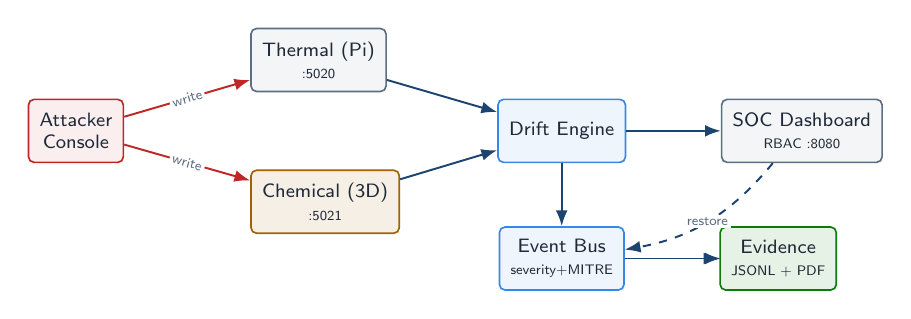
\begin{tikzpicture}[node distance=5mm and 12mm]
\node[red] (atk) {Attacker\\Console};
\node[box, right=16mm of atk, yshift=9mm] (pi) {Thermal (Pi)\\\tiny :5020};
\node[chemb, right=16mm of atk, yshift=-9mm] (chem) {Chemical (3D)\\\tiny :5021};
\node[acc, right=14mm of pi, yshift=-9mm] (eng) {Drift Engine};
\node[acc, below=8mm of eng] (bus) {Event Bus\\\tiny severity+MITRE};
\node[box, right=12mm of eng] (dash) {SOC Dashboard\\\tiny RBAC :8080};
\node[goodb, right=12mm of bus] (ev) {Evidence\\\tiny JSONL + PDF};
\draw[flr](atk)--node[lbl,sloped]{write}(pi);
\draw[flr](atk)--node[lbl,sloped]{write}(chem);
\draw[fl](pi)--(eng); \draw[fl](chem)--(eng);
\draw[fl](eng)--(bus); \draw[fl](eng)--(dash); \draw[fl](bus)--(dash.west|-bus); \draw[fl](bus)--(ev);
\draw[fl,dashed](dash) to[bend left=20] node[lbl]{restore} (bus);
\end{tikzpicture}
\end{center}
\vspace{2pt}
{\small Every detector emits one \code{Event}. On emit the bus enriches it (\hl{severity, MITRE,
identity, sequence}) and fans out to the evidence log, the poll buffer and live subscribers.
Events carry \code{details.site} --- so two plants share one timeline.}
\end{frame}

% ---------------- DETECTION ----------------
\begin{frame}{Detection: six named PLC mutations}
\begin{columns}[T]
\begin{column}{0.62\textwidth}
\footnotesize
\renewcommand{\arraystretch}{1.25}
\begin{tabularx}{\textwidth}{@{}l>{\raggedright\arraybackslash}X l@{}}
\toprule
\textbf{Mutation} & \textbf{Meaning} & \textbf{MITRE}\\ \midrule
condition stripping & safety input removed & T0889\\
logic inversion & comparator flipped & T0889\\
coil hijack & output repointed & T0889\\
rung injection & backdoor rung added & T0843\\
setpoint drift & threshold changed & T0836\\
register change & raw Modbus write & T0855\\
\bottomrule
\end{tabularx}
\end{column}
\begin{column}{0.38\textwidth}
\begin{block}{Two surfaces}
\small \textbf{Structural} --- canonicalize \& diff the L5X rung-by-rung.\\[3pt]
\textbf{Register} --- diff live holdings/coils vs the signed snapshot.
\end{block}
{\color{muted}\footnotesize A harmless re-export hashes identically $\Rightarrow$ no alert. A real change is caught on the first 1-second scan.}
\end{column}
\end{columns}
\end{frame}

% ---------------- LIFECYCLE ----------------
\begin{frame}{Every attack runs the full lifecycle}
\begin{center}
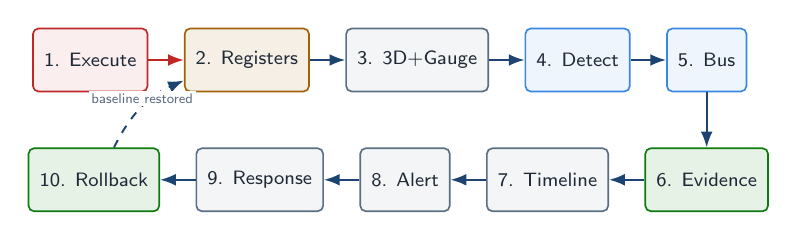
\begin{tikzpicture}[node distance=3mm and 4.5mm, every node/.style={font=\tiny\sffamily}]
\node[red] (a){1. Execute};
\node[chemb,right=of a](b){2. Registers};
\node[box,right=of b](c){3. 3D+Gauge};
\node[acc,right=of c](d){4. Detect};
\node[acc,right=of d](e){5. Bus};
\node[goodb,below=7mm of e](f){6. Evidence};
\node[box,left=of f](g){7. Timeline};
\node[box,left=of g](h){8. Alert};
\node[box,left=of h](i){9. Response};
\node[goodb,left=of i](j){10. Rollback};
\draw[flr](a)--(b);\draw[fl](b)--(c);\draw[fl](c)--(d);\draw[fl](d)--(e);
\draw[fl](e)--(f);\draw[fl](f)--(g);\draw[fl](g)--(h);\draw[fl](h)--(i);\draw[fl](i)--(j);
\draw[fl,dashed](j) to[bend left=20] node[lbl,above]{baseline restored}(b);
\end{tikzpicture}
\end{center}
\vspace{4pt}
{\small On a live stage you can point to \emph{every} stage on screen: the attacker fires, the
registers move, the gauge/3D reacts, the alert appears with a MITRE badge, evidence is logged,
and one click restores the approved baseline.}
\end{frame}

% ---------------- ATTACKS ----------------
\begin{frame}{Twelve real attacks --- over genuine channels}
\begin{columns}[T]
\begin{column}{0.48\textwidth}
\textbf{\color{navy}Site A --- Thermal (7)}
\begin{itemize}\footnotesize
  \item Setpoint drift, force coil \hfill{\color{muted}Modbus}
  \item Logic inversion, condition stripping
  \item Coil hijack, rung injection \hfill{\color{muted}Program}
  \item DDoS flood \hfill{\color{muted}T0814}
\end{itemize}
\end{column}
\begin{column}{0.52\textwidth}
\textbf{\color{navy}Site B --- Chemical (5, blast last)}
\begin{enumerate}\footnotesize
  \item Quality Sabotage \hfill{\color{muted}stealth / colour}
  \item Feed Pump Trip \hfill{\color{muted}level drains}
  \item Tank Overfill \hfill{\color{muted}level rises + trip}
  \item E-Stop Injection \hfill{\color{muted}plant halts}
  \item \textbf{\color{critical}Pressure Redline --- BLAST}
\end{enumerate}
\end{column}
\end{columns}
\vspace{6pt}
\begin{center}\small
Each chemical attack drives a \hl{distinct} live signature --- no two look alike on the gauges,
detection feed or timeline.
\end{center}
\end{frame}

% ---------------- 3D DEMO ----------------
\begin{frame}{The showpiece: a live 3D chemical reactor}
\begin{columns}[T]
\begin{column}{0.55\textwidth}
\begin{itemize}\small
  \item The real Fortiphyd \hl{GRFICS Unity} reactor, embedded live in the SOC dashboard.
  \item Driven entirely by \hl{live process data} --- no scripted animation.
  \item The demo escalates: stealth sabotage $\rightarrow$ starvation $\rightarrow$ overfill $\rightarrow$ halt $\rightarrow$ \hl{the reactor blasts}.
  \item Cinematic letterbox framing; the blast is \hl{guaranteed} to fire (pressure to the ceiling in $\sim$13\,s).
\end{itemize}
\end{column}
\begin{column}{0.45\textwidth}
\begin{block}{Honest engineering}
\small The Unity binary is pre-compiled; its process animations are what the binary maps. \emph{All}
per-attack distinctiveness is guaranteed on the live \hl{SOC gauges + detection}, with a documented
recompile path to unlock full 3D animation.
\end{block}
\end{column}
\end{columns}
\end{frame}

% ---------------- DASHBOARD ----------------
\begin{frame}{Production-grade SOC dashboard}
\begin{columns}[T]
\begin{column}{0.5\textwidth}
\begin{itemize}\small
  \item \hl{Risk Score} --- explainable 0--100 + band
  \item \hl{Attack Timeline} --- severity-coloured, site-filtered
  \item \hl{System Health} --- per-site status rollup
  \item \hl{Rollback status} --- integrity + drift + restore
\end{itemize}
\end{column}
\begin{column}{0.5\textwidth}
\begin{itemize}\small
  \item \hl{Live trend sparklines} --- rolling telemetry
  \item \hl{Animated SCADA mimic} with pinned MITRE badges
  \item \hl{Site selector} --- Thermal / Chemical / All
  \item \hl{Signed forensic PDF} --- per site, on demand
\end{itemize}
\end{column}
\end{columns}
\vspace{6pt}
\begin{center}\small
Polling, not WebSockets --- \hl{deliberately}, for live-demo robustness.
\end{center}
\end{frame}

% ---------------- RBAC ----------------
\begin{frame}{Capability-based RBAC --- six OT/ICS roles}
\footnotesize
\renewcommand{\arraystretch}{1.25}\setlength{\tabcolsep}{5pt}
\begin{center}
\begin{tabular}{@{}l l c c c c c c@{}}
\toprule
\textbf{Role} & \textbf{Scope} & ack & ack all & baseline & net & safe & evidence\\ \midrule
Operator & control room & \checkmark & \checkmark & & & & \\
Control Engineer & PLC program & \checkmark & \checkmark & \checkmark & & \checkmark & \\
Network Engineer & infrastructure & \checkmark & \checkmark & & \checkmark & & \\
SOC Analyst & oversight & \checkmark & \checkmark & & \checkmark & \checkmark & \checkmark\\
Vendor / OEM & read-only & & & & & & \\
CISO & full authority & \checkmark & \checkmark & \checkmark & \checkmark & \checkmark & \checkmark\\
\bottomrule
\end{tabular}
\end{center}
\vspace{4pt}
{\small Gated by \hl{capability}, not rank --- roles have different \emph{scopes}. Enforced
server-side (HTTP 403) \emph{and} client-side. Vendor is read-only + monitored; CISO is full.}
\end{frame}

% ---------------- VERIFICATION ----------------
\begin{frame}{Verified, not hand-waved}
\begin{columns}[T]
\begin{column}{0.46\textwidth}
\begin{block}{154 automated checks}
\small Nine integration suites spin up real servers on ephemeral ports and exercise real
HTTP/Modbus paths --- integration, not unit tests.
\end{block}
\end{column}
\begin{column}{0.54\textwidth}
\footnotesize
\begin{tabularx}{\textwidth}{@{}Xr@{}}
bus \textbullet\ l5x \textbullet\ plant & 45\\
drift (6 mutations) & 18\\
agent \textbullet\ dashboard (RBAC) \textbullet\ attacker & 35\\
grfics (5 distinct chemical attacks) & 36\\
multisite (unified feed, both sites) & 20\\
\midrule
\textbf{Total} & \textbf{154}\\
\end{tabularx}
\end{column}
\end{columns}
\vspace{6pt}
\begin{center}\small
Every attack's \hl{detection, severity, MITRE and site-tag} is asserted. MITRE IDs are
\hl{verified against the live ICS matrix}; where none fits, it is honestly \code{N/A}.
\end{center}
\end{frame}

% ---------------- WHY WE WIN ----------------
\begin{frame}{Why LogicWard wins the room}
\begin{columns}[T]
\begin{column}{0.5\textwidth}
\textbf{\color{navy}Differentiators}
\begin{itemize}\small
  \item \hl{Multi-site, multi-vendor} on one fabric --- rare in a demo.
  \item A \hl{live 3D digital twin} that reacts to real attacks.
  \item \hl{Explainable} detection + \hl{verified} MITRE mapping.
  \item \hl{Full lifecycle} on screen, ending in one-click rollback.
\end{itemize}
\end{column}
\begin{column}{0.5\textwidth}
\textbf{\color{navy}Enterprise-ready signals}
\begin{itemize}\small
  \item Capability RBAC for six real OT roles.
  \item Signed baseline + forensic PDF (audit trail).
  \item Risk score + health + timeline (SOC language).
  \item Process-agnostic --- water / substation next.
\end{itemize}
\end{column}
\end{columns}
\end{frame}

% ---------------- ROADMAP ----------------
\begin{frame}{Roadmap}
\begin{itemize}
  \item \hl{Structured-Text program drift} for the chemical PLC --- same six mutations, second parser.
  \item \hl{Unity recompile} to hook liquid level / colour / e-stop strobes to the published JSON keys.
  \item \hl{New site profiles} --- water treatment, electrical substation --- as drop-in plugins.
  \item \hl{ML-assisted risk scoring} layered above the explainable rule-based core.
\end{itemize}
\vspace{10pt}
\begin{block}{}
\centering One detection fabric, many plants. \hl{Research-grade. Demonstration-ready.}
\end{block}
\end{frame}

% ---------------- CLOSE ----------------
{
\setbeamertemplate{background}{\color{navy}\rule{\paperwidth}{\paperheight}}
\setbeamercolor{normal text}{fg=white}
\begin{frame}[plain]
\vspace{1.4cm}
{\color{accent}\rule{0.4\textwidth}{2.5pt}}\\[10pt]
{\Huge\bfseries\color{white} LogicWard}\\[8pt]
{\large\color{page} Let's watch a reactor get attacked --- and caught.}\\[18pt]
{\color{page}\small SOC dashboard \code{:8080} \quad\textbullet\quad Attacker console \code{:9090}}\\[6pt]
{\color{muted}\footnotesize Thank you.}
\end{frame}
}

\end{document}
